% !TeX program = pdfLaTeX
\documentclass[12pt]{article}
\usepackage{amsmath}
\usepackage{graphicx,psfrag,epsf}
\usepackage{enumerate}
\usepackage{natbib}
\usepackage{textcomp}
\usepackage[hyphens]{url} % not crucial - just used below for the URL
\usepackage{hyperref}
\providecommand{\tightlist}{%
  \setlength{\itemsep}{0pt}\setlength{\parskip}{0pt}}

%\pdfminorversion=4
% NOTE: To produce blinded version, replace "0" with "1" below.
\newcommand{\blind}{0}

% DON'T change margins - should be 1 inch all around.
\addtolength{\oddsidemargin}{-.5in}%
\addtolength{\evensidemargin}{-.5in}%
\addtolength{\textwidth}{1in}%
\addtolength{\textheight}{1.3in}%
\addtolength{\topmargin}{-.8in}%

%% load any required packages here



% Pandoc citation processing

\usepackage{amsmath}
\usepackage{amsfonts}
\usepackage{booktabs}
\usepackage{makecell}
\usepackage[usenames, dvipsnames]{color}
\usepackage{multirow}
\usepackage{comment}
\usepackage{booktabs}
\usepackage{longtable}
\usepackage{array}
\usepackage{wrapfig}
\usepackage{float}
\usepackage{colortbl}
\usepackage{pdflscape}
\usepackage{tabu}
\usepackage{threeparttable}
\usepackage{threeparttablex}
\usepackage[normalem]{ulem}
\usepackage{xcolor}
\newcommand{\beginsupplement}{\setcounter{table}{0} \renewcommand{\thetable}{S\arabic{table}}\setcounter{figure}{0} \renewcommand{\thefigure}{S\arabic{figure}}}
\usepackage{booktabs}
\usepackage{longtable}
\usepackage{array}
\usepackage{multirow}
\usepackage{wrapfig}
\usepackage{float}
\usepackage{colortbl}
\usepackage{pdflscape}
\usepackage{tabu}
\usepackage{threeparttable}
\usepackage{threeparttablex}
\usepackage[normalem]{ulem}
\usepackage{makecell}
\usepackage{xcolor}

\begin{document}


\def\spacingset#1{\renewcommand{\baselinestretch}%
{#1}\small\normalsize} \spacingset{1}


%%%%%%%%%%%%%%%%%%%%%%%%%%%%%%%%%%%%%%%%%%%%%%%%%%%%%%%%%%%%%%%%%%%%%%%%%%%%%%

\if0\blind
{
  \title{\bf How will we move: Modeling Climate-driven Age-specific
Displacement Migration}

  \author{
        Mathew E. Hauer \thanks{Thanks y'all!} \\
    Department of Sociology, Florida State University\\
     and \\     Sunshine Jacobs \\
    Department of Sociology, Florida State University\\
      }
  \maketitle
} \fi

\if1\blind
{
  \bigskip
  \bigskip
  \bigskip
  \begin{center}
    {\LARGE\bf How will we move: Modeling Climate-driven Age-specific
Displacement Migration}
  \end{center}
  \medskip
} \fi

\bigskip
\begin{abstract}
Global population projections show widespread ageing by century's end.
The well-known relationship between age and migration propensity
suggests more youthful populations are more likely to migrate than older
populations. Yet relatively little research explores the important
implication of ageing on human mobility in a changing climate, most
likely driven by a paucity of migration data to comprehensively
investigate the age structure of environmental migration. Here, we
propose a displacement migration model to estimate age-specific
migration probabilities. We combine a statistical outlier detection
algorithm to first identify major environmental displacement events in
US counties since 1980. Our findings suggests populations under age 60
are most likely to migrate after an environmental event, increasing with
the size of displacement, validating many findings in the migration
literature. We then build a flexible one-dimensional, age-specific
displacement model based on these findings with estimation errors
suggesting reasonable accuracy. Our proposed displacement model can be
readily deployed to model prospective climate migration.
\end{abstract}

\noindent%
{\it Keywords:} Climate Change, Human Migration, Demography
\vfill

\newpage
\spacingset{1.45} % DON'T change the spacing!

\newpage

\hypertarget{introduction}{%
\section{Introduction}\label{introduction}}

Environmental migration is an increasingly important concern in a
warming world
\citep{blackClimateChangeMigration2011, findlayMigrantDestinationsEra2011, boas2019climate}.
Some research suggests there could be as many as 140 million climate
migrants by the middle of this century \citep{rigaud2018groundswell},
suggesting environmental and climate migration will remain an important
concern this century.

Although there is increasing interest in environmental migration, most
migration research suffers from two key limitations. First, most studies
on environmental migration use case study approaches employing either a
single country or a single environmental event. Using case studies makes
sense, especially with the ever lengthening list of major environmental
events that can be coupled with good migration data. For instance, there
are now a multitude of studies on Hurricane Katrina in New Orleans in
2005 (e.g.,
\citep{fussellRaceSocioeconomicStatus2010, fussellRecoveryMigrationCity2014, thiedeHurricaneKatrinaWho2013, groen2010going}),
a growing number of studies on Hurricane Maria in Puerto Rico in 2017
\citep{alexander2019impact, dewaard2020out, acosta2020quantifying}, and
many studies on natural disasters
\citep{kayastha1985flood, loebach2016household, paul2005evidence, mallick2014population}.
Few studies attempt more systematic analyses of environmental migration
(see \citet{obokata2014empirical}, \citet{hunter2015environmental},
\citet{hoffmann2020meta} for broader reviews of environmental). This has
lead to a patchwork of our understanding of environmental migration,
with environmental migration signals often showing conflicting findings
\citep{hoffmann2020meta}.

Second, most studies on environmental migration focus on population
aggregates, examining total population changes (e.g.
\citet{luUnveilingHiddenMigration2016}, \citet{hauer2020evacuees},
\citet{nawrotzki2013rainfall}). Yet migration propensity has a
well-known age gradient where the most likely to migrate are young
adults and the least likely are older adults. We know from some case
studies that typical migration patterns manifest after an environmental
event
\citep{thiedeHurricaneKatrinaWho2013, groen2010going, keenan2020resilience},
but these case studies involve some of the most destructive hurricanes
in US history. The extent to which typical migration patterns manifest
after smaller, less destructive events is presently unknown.

These two shortcomings related to isolated case studies and total
population are important limitations on our ability to predict future
environmental migration. The parallels between historic environmental
migration and future climate migration form the backbone of most
prospective analyses of climate migration
\citep{rigaud2018groundswell, hauerMigrationInducedSealevel2017, chen2018coastal, xu2020future}.
Yet many of these prospective analyses rely on individual case studies
\citep{chen2018coastal, robinson2020modeling}, general migration theory
\citep{hauerMigrationInducedSealevel2017, bell2021migration}, or heavy
modeling of urban/rural populations
\citep{rigaud2018groundswell, gao2020mapping}. Conspicuously missing
from these models are attempts to capture the well-known relationship
between migration propensity and age. Furthermore, while general
migration theory and individual case studies are important and useful,
the efficacy of using them for prospective analyses of climate migration
is questionable.

In this article, we rectify these shortcomings of environmental
migration studies. To overcome the limitation of case studies, we couple
a statistical outlier \citep{chen1993joint} technique with nearly 40
years of population data in approximately 3000 US counties (for
approximately 120k county-years) to search for environmental events
associated with large population declines. We then use the Spatial
Hazard Events and Losses Database for the United States
(SHELDUS)\footnote{available at \url{http://www.sheldus.org}} to ensure
the outliers we detect are associated with an environmental hazard
rather than other factors, like a factory closing. This search provides
a relatively large and varied historical pool of significant
environmental hazards, overcoming the limitations of isolated case
studies. From this pool of displacement events, we overcome the second
limitation regarding a limitation to population aggregates by building a
parsimonious, one-dimensional, age-specific displacement model. We link
total population declines with changes in age-specific cohort change
ratios to produce a predictive model of age-sex population changes in
the face of an environmental hazard.

\hypertarget{environmental-migration}{%
\section{Environmental Migration}\label{environmental-migration}}

\hypertarget{methods}{%
\section{Methods}\label{methods}}

First, we describe the data sets we used. Second, the methodology for
detecting statistical outliers in time series. Finally, we describe the
creation of our flexible one-dimensional, age-specific displacement
model.

\hypertarget{data-sets}{%
\subsection{Data sets}\label{data-sets}}

We use two primary datasets: the National Vital Statistics System (NVSS)
U.S. Census Populations with Bridged Race Categories data set\footnote{Data
  can be downloaded here:
  \url{https://seer.cancer.gov/popdata/download.html}} and the Spatial
Hazard Events and Losses Database for the United States (SHELDUS).

The NVSS Bridged Race Categories data set harmonizes racial
classifications across disparate time periods to allow population
estimates to be sufficiently comparable across space and time.
Importantly, all county boundaries are rectified to be geographically
consistent across all time periods. We use the the 1969-2018 dataset
which includes annual population estimates in five year age groups
(0-4,\ldots, 85+), two sex groups (male and female), and three race
groups (White, Black, Other).

In our statistical outlier analysis (detailed below), we only consider
counties created prior to 2000 and contained in the NVSS data. NVSS
aggregated all counties in Hawaii to the state-level in the 1969-2018
NVSS bridged race data and we exclude them from our analysis. Several
counties were created after 2000 (most notably is Broomfield County,
Colorado). The 15 counties excluded from our analysis due to boundary
changes or other reasons are Hoonah-Angoon Census Area AK 02105,
Kusilvak Census Area AK 02158, Prince of Wales-Outer Ketchikan Census
Area AK 02201, Skagway-Hoonah-Angoon Census Area AK 02232,
Wrangell-Petersburg Census Area AK 02280, Adams County CO 08001, Boulder
County CO 08013, Broomfield County CO 08014, Jefferson County CO 08059,
Weld County CO 08123, Hawaii County HI 15001, Honolulu County HI 15003,
Kalawao County HI 15005, Kauai County HI 15007, and Maui County HI
15009.

We use these data in two separate steps. In our statistical outlier
analysis, we aggregate all county-level estimates into annual total
population estimates for each county for the period 1969-2016. The
historical population estimates prior to 1980 display unusual
volatility, so we consider only the time periods 1980-2018. We use the
NVSS population estimates disaggregated by age/sex to calculate
cohort-change ratios, which we describe below.

The second data source we use is SHELDUS. SHELDUS is a county-level
hazard data set for the US which contains information about the direct
losses (property and crop losses, injuries, and fatalities) caused by a
hazard event (thuderstorms, hurricanes, floods, wildfires, tornados,
flash floods, earthquakes, etc.) for the period 1960 to the present. We
use this database to ensure the county time periods we identify as
statistical outliers with population losses contain experienced an
environmental hazard in that county-year. This is to ensure the outlier
population losses that we detect are associated with a hazard rather
than other forces, such as economic forces.

\hypertarget{statistical-outlier-detection}{%
\subsection{Statistical Outlier
Detection}\label{statistical-outlier-detection}}

We use a statistical time series outlier detection algorithm
\citep{chen1993joint}, implemented in the R programming language
\citep{rcore} via the tsoutliers package \citep{tsoutliers2019}. This
algorithm iteratively uses ARIMA models to 1) identify potential
outliers and 2) refit the ARIMA with the outliers removed to produce a
counter-factual time series. Here we briefly summarize and describe the
method.

Often, the behavior of a time series can be described and summarized in
ARIMA models. If a series of values, \(y_t^*\), is subject to \(m\)
interventions or outliers at time points \(t_1,t_2,…,t_m\) with weights
\(\omega\) then \(y_t^*\) can be defined as

\begin{equation}
\label{eq:arima}
y_t^* = \sum_{j=1}^{m} \omega_jL_j(B)I_t(t_j) + \frac{\theta(B)}{\phi(B)\alpha(B)}a_t 
\end{equation}

Where \(I_t(t_j)\) is an indicator variable with a value of 1 at
observation \(t_j\) and where the \(j\)th outlier arises,\\
\(\phi(B)\) is an autoregressive polynomial with all roots outside the
unit circle,\\
\(\theta(B)\) is a moving average polynomial with all roots outside the
unit circle,\\
and \(\alpha(B)\) is an autoregressive polynomial with all roots on the
unit circle.

We examine three types of outliers at time point \(t_m\):\\
1. additive outliers (AO), defined as \(L_j(B)=1\);\\
2. level shift outliers (LS), defined as \(L_j(B) = 1/(1-B)\); and\\
3. temporary change outliers (TC), defined as
\(L_j(B) = 1/(1-\delta B)\) where \(\delta\) is equal to 0.7.

Colloquially, additive outliers arise when a single event causes the
time series to unexpectedly increase/decrease for a single time period;
level shift outliers arise when an event causes the time series to
unexpectedly increase/decrease for multiple time periods; and temporary
change outliers arise when an event causes the time series to
unexpectedly increase/decrease with lingering effects that decay over
multiple time periods.

An outlier is detected with the estimated residuals using a regression
equation

\begin{equation}
\label{eq:residuals}
\pi(B)y_t^* \equiv \hat{e} = \sum_{j=1}^m \omega_j \pi(B)L_j(B)I_t(t_j) + a_t
\end{equation} where \(\pi(B)=\sum_{i=o}^{inf} \pi_iB^i\).

Equations \ref{eq:arima} and \ref{eq:residuals} allow for an automatic
detection of outliers iterated over a two-stage process.

In stage 1, outliers are located. First, an ARIMA model is fit to the
time series using the \texttt{forecast} package in R
\citep{Rforecast, hymdman2008} where the best performing ARIMA model is
selected based on the Bayesian information criterion (BIC). Next, the
residuals from the forecast are checked for their significance using
equation \ref{eq:residuals} where only outliers above a critical
\emph{t}-static are considered ``true'' outliers (\(|\tau| \geq 4\);
p-value \textless{} 0.000063). We chose this threshold to minimize the
probability of committing a Type I error (or claiming an outlier is true
when it is in fact not). Finally, two additional rules are implemented:
If multiple outliers are detected at the same time point, only the most
significant outlier is selected and if outliers of the same type at
consecutive time periods are detected, only the outlier with highest
\emph{t}-statistic is selected.

In stage 2, outliers are removed from the time series and a new ARIMA
model is chosen and fit. The selection of the initial ARIMA model could
have been affected by the presence of the outliers, making some outliers
spuriously identified. To correct for this, a new ARIMA model is fit
accounting for additional regression effects in equation \ref{eq:arima}
from the list of candidate outliers identified in stage 1, effectively
removing the outliers from the time series. Each outlier is then
reassessed under the new model and those outliers that are no longer
significant are removed.

These two stages are then iterated until no additional outliers are
detected.

\begin{figure}
\centering
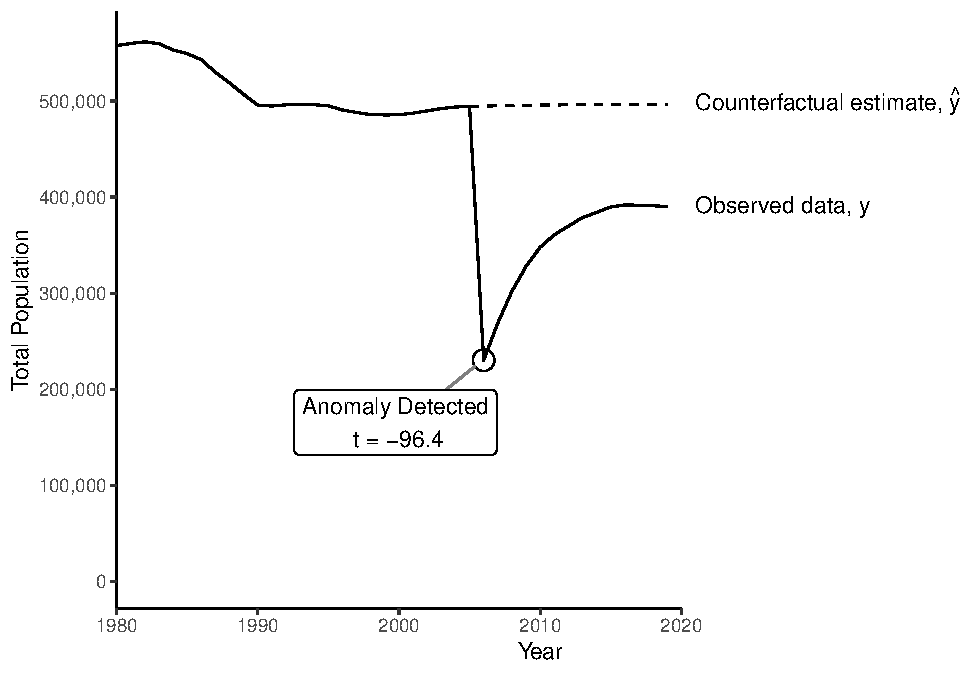
\includegraphics{manuscript_files/figure-latex/ToyExample-1.pdf}
\caption{\textbf{An example of outlier detection using Hurricanes Katrina and Rita in Orleans Parish Louisiana in 2005.}
Hurricane Katrina struck Louisiana in 2005 and we use it as a toy
example to illustrate our approach. This figure shows the annual time
series of total population in Orleans Parish between 1980 and 2019.
Between 1990 and 2005, Orleans Parish total population changed from 495k
to 494k, suggesting a possible `plateau' in the population (illustrated
with the dotted `counterfactual'). Hurricane Katrina and the widespread
population loss of more than 200k people represent a very strong outlier
(t=-96.39). \label{explanationfigure}}
\end{figure}

\textbf{\autoref{explanationfigure}} shows a toy example for outlier
detection in a time series using the example of Hurricane Katrina in
Orleans Parish. On August 23 2005, Hurricane Katrina, a category 5
hurricane, struck southern Louisiana causing widespread damage and
destruction in Orleans Parish in particular. The displacement from the
Hurricane and the federal response were well documented
\citep{horiDisplacementDynamicsSouthern2009, fussellRecoveryMigrationCity2014}
and Census estimates suggest Orleans Parish lost more than 200,000
residents between 2005 and 2006. What would have been Orleans'
population estimate had Hurricane Katrina \emph{not} occurred? A simple
counter-factual estimate might keep population size just under 500,000
people (\(\hat{y}\)).

In the Hurricane Katrina example, we have knowledge of the impact of
Hurricane Katrina after the fact or ex-post-facto in order to create the
counter-factual time series \(\hat{y}\). But is this outlier detectable
without knowledge of the Hurricane Katrina? In other words, can we
detect the reduction of Orleans Parish's population between 2005 and
2006 using only the time series? Absolutely. The tsoutliers package
identifies 2006 as an extremely strong level-shift outlier
(\emph{t}-stat = -96.39). The real world is hardly this simplified where
a direct intervention is known, is large, and is testable. However, by
using SHELDUS to verify environmental damages associated with large
population declines, we can be confident the population shifts we detect
are at least partially attributable to an environmental hazard.

\hypertarget{flexible-one-dimensional-age-specific-displacement-model}{%
\subsection{Flexible one-dimensional, age-specific displacement
model}\label{flexible-one-dimensional-age-specific-displacement-model}}

We search all US counties for negative statistical outliers (indicating
population losses) between 1980 and 2018. We detect population losses of
magnitude 4\(\sigma\) or greater. We then searched the SHELDUS database
to see if these county-years experienced per capita hazardous losses in
excess of the 50th percentile. Four county-periods either were not in
the SHELDUS database or experienced per capita hazard losses below the
50th percentile. Additionally, one county-period contained age-sex
groups with 0 people, necessitating exclusion. These 48 environmental
events include tornados, wind damage, winter weather, earthquakes,
flooding, tropical cyclones, hail, and other environmental hazards.

With 48 county-periods exhibiting large population declines after
verified hazard losses, across over nearly 40 years and across a wide
variety of environmental hazards, we are able to overcome the first
limitation of previous environmental migration modelling: that of
isolated case studies of individual environmental events. With this
large sample of environmental displacement, we next overcome the second
limitation: that of only examining total population. To examine
environmental migration across age, we build a flexible,
one-dimensional, age-specific displacement model.

To link population displacement with age-specific population changes, we
calculate cohort-change ratios in each county. Using the demographic
accounting equation, the population at some time period \emph{t} is
equal to the
\(Pop_{t-1} + Births_{t-1} - Deaths_{t-1} + Migrants_{{t-1},in} - Migrants_{{t-1},out}\).
For all age groups older than 0, \(Births_{t-1}\) must be 0.

The calculation of a cohort-change ratio, as its name suggests, is
relatively straightforward:

\[ 
CCR_{x,t}  =  \frac {_nP_{x,t}} {_nP_{x-y,t-y}}
\]

Where \(_nP_{x,t}\) is the population aged \(x\) to \(x+n\) in time
\(t\) and \(_nP_{x-y,t}\) is the population aged \(x-y\) to \(x+n-y\) in
time \(t\) where \(y\) refers to the time difference between time
periods. Since mortality must decrement a population, any CCR above 1.0
implies a net-migration rate in excess of the mortality rate, and a
growing population.

We build the following model based on the relationship between the
change in CCRs at age \(x\), \(\Delta CCR_x = CCR_{x,t} / CCR_{x,t-1}\),
and the percentage decline in the total population compared to the
counter-factual in the outlier detection method,
\(\Delta P_t = \hat{P_t} / P_t\):

\[
log(\Delta CCR_x) = a_x + b_xh
\]

Here, \(h\) is the log(\(\Delta P_t\)) and shows a linear relationship
with the logarithm of the change in CCRs by age. \(x\) refers to
five-year age groups: 0-4, 5-9,\ldots, 85+. This is a similar model and
approach to Wilmoth et al's \citeyearpar{wilmoth2012flexible} flexible,
one-dimensional mortality model based on the linearity between
age-specific mortality rates and infant-mortality. \textbf{Table 1}
depicts the correlation coefficients between log(\(\Delta CCR_x\)) and
log(\(\Delta P_t\)). The age groups with the lowest correlation
coefficients are young adult males aged 20-39 and those in the
open-ended age interval (80+), suggesting these age/sex groups react to
environmental signals the least predictably.

\begin{table}

\caption{\label{tab:correltable}\textbf{Correlation coefficients of changes in Cohort Change Ratios vs. Total Population Change (n=48).}}
\centering
\begin{tabular}[t]{lrr}
\toprule
Age Group & Male & Female\\
\midrule
0-4 & 0.931 & 0.944\\
5-9 & 0.954 & 0.934\\
10-14 & 0.963 & 0.965\\
15-19 & 0.806 & 0.930\\
20-24 & 0.650 & 0.919\\
\addlinespace
25-29 & 0.710 & 0.934\\
30-34 & 0.752 & 0.959\\
35-39 & 0.874 & 0.975\\
40-44 & 0.936 & 0.964\\
45-49 & 0.971 & 0.963\\
\addlinespace
50-54 & 0.969 & 0.977\\
55-59 & 0.965 & 0.958\\
60-64 & 0.896 & 0.888\\
65-69 & 0.809 & 0.912\\
70-74 & 0.937 & 0.826\\
\addlinespace
75-79 & 0.839 & 0.795\\
80+ & 0.478 & 0.651\\
\bottomrule
\end{tabular}
\end{table}

\textbf{\autoref{CCRfig}} shows the relationship for selected age-groups
between log(\(\Delta CCR_x\)) and log(\(\Delta P_t\)). Here we can see
the near linear relationship between the percentage reduction in the
population and the percentage reduction in \(CCR_x\). Note the two
county-years with the greatest reductions in total population refer to
Louisiana counties most impacted by Hurricane Katrina.

\begin{figure}
\centering
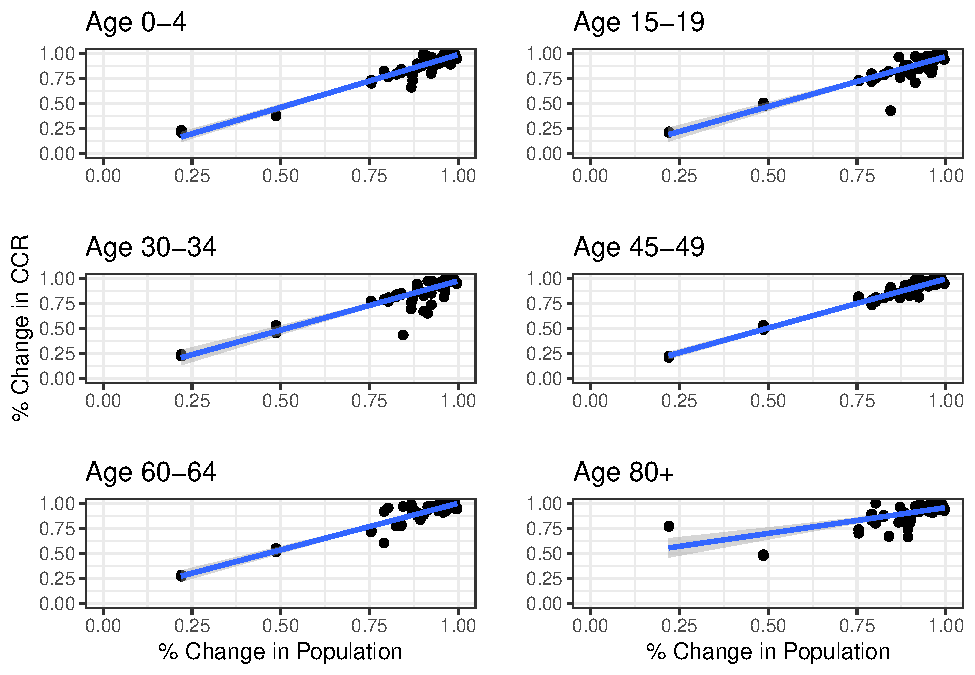
\includegraphics{manuscript_files/figure-latex/CCRfig-1.pdf}
\caption{\textbf{Age-specific changes in cohort-change ratios ($\Delta CCR_x$) vs. change in total population ($\Delta P_t$).}
\label{CCRfig}}
\end{figure}

\hypertarget{environmental-migration-estimation-using-the-fitted-model}{%
\subsection{Environmental Migration estimation using the fitted
model}\label{environmental-migration-estimation-using-the-fitted-model}}

Using \(h=log(\Delta P_t)\), we can estimate age-specific changes in
CCRs after an environmental event by simply applying the following
formula:

\[\hat{CCR_{x,t}} = CCR_{x,t-1} \cdot e^{\hat\beta_xh}\] Where
\(e^{\hat\beta_xh}\) provides the percentage change in \(CCR_x\) based
on the log(\(\Delta{P_t}\)).In this case, we drop the intercept (\(a\))
from the estimation procedure to ensure a 0\% decline in population
yields a corresponding 0\% change in the CCR. Simply multiplying the
result from the model with the CCR in the year prior yields the
anticipated change in the CCR. These changes in CCRs can then be applied
to any time series of population values to generate an anticipated
population.

\begin{figure}
\centering
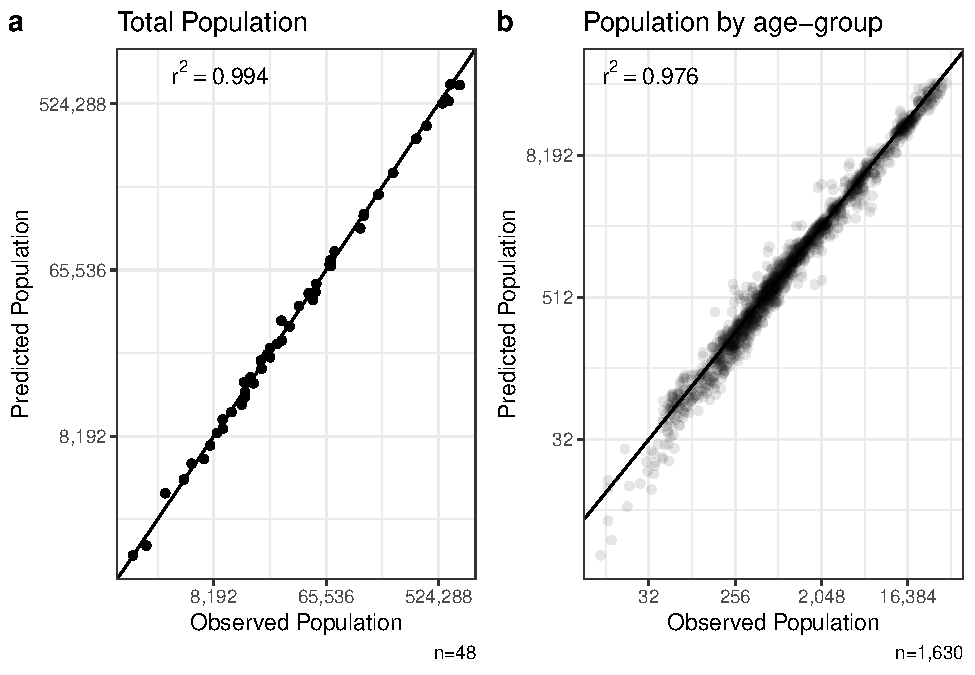
\includegraphics{manuscript_files/figure-latex/evalfig-1.pdf}
\caption{\textbf{Relationship between predicted populations using our model and observed populations in the 48 counties in our selection.}
(a) shows the total population and (b) shows the populations for each
age/sex group. The diagonal solid line is y=x. The model produces good
fits for both the total population and by age/sex group.
\label{EvalFig}}
\end{figure}

\textbf{\autoref{EvalFig}} shows the accuracy of the our fitted,
one-dimensional model. We estimate the predicted population using the
equation outlined above and then compare against the observed
population. Regarding total population in our 48 counties, our model
performs well with an \(r^2\) value of 0.994 and performs well
regardless of population size. Regarding each individual \(P_x\) group,
our model performs slightly worse, but still performs quite well with an
\(r^2\) of 0.976. And just like with total population, the accuracy of
our model does not depend on population size.

\hypertarget{conclusion}{%
\section{Conclusion}\label{conclusion}}

In this paper we introduced a flexible, one-dimensional age-specific
migration model using a statistical outlier search algorithm. We
searched over 3,000 US counties for significant population declines and
then cross referenced our outliers with data from SHELDUS to eliminate
spurious outliers. We then built and evaluated a predictive model of
age-sex specific population change attributable to environmental events.

By using a more systematic analyses we are able to consider
environmental migration clarifying the nature of environmental migration
beyond individual case studies. Populations 60 and younger are more
likely to migrate while those older than 60 could be demographically
trapped.

We then built and evaluated a predictive model of age-sex specific
population change attributable to environmental events allowing us to
further analyze the possible displacement consequences of migration
propensity and age. This displacement model predicts total population
declines and the respective age/sex group changes.

The climate migration literature is replete with aggregate models of
climate migration and displacement. However, our work underscores the
importance of including basic demographic characteristics in prospective
models of climate migration.

\newpage

\bibliographystyle{agsm}
\bibliography{mybibfile}

\end{document}
